% Configurazione
\documentclass[12pt, a4paper]{report}

\usepackage[table,xcdraw]{xcolor}
\usepackage{graphicx}
\usepackage{xcolor}
\usepackage{titlesec}
\usepackage{amssymb}
\usepackage{hyperref}
\usepackage{float}
\usepackage{fancyhdr}
\usepackage{geometry}
\usepackage{longtable}
\usepackage[italian]{babel}
\usepackage{array}
\newcolumntype{L}[1]{>{\raggedright\arraybackslash}p{#1}}
\newcolumntype{C}[1]{>{\centering\arraybackslash}p{#1}}
\newcolumntype{R}[1]{>{\raggedleft\arraybackslash}p{#1}}

\hypersetup{
    colorlinks=true,
    linkcolor=black,
    urlcolor=blue,
}

\geometry{
  top=30mm,
  bottom=30mm,
  left=30mm,
  right=30mm,
}

\pagestyle{fancy}
\lhead{}
\lfoot{Piano di Qualifica}
\cfoot{}
\rfoot{\thepage}
\renewcommand{\headrulewidth}{0.4pt}
\renewcommand{\footrulewidth}{0.4pt}
\setlength{\headheight}{16pt}

\fancypagestyle{firstpage}{%
  \renewcommand{\headrulewidth}{0pt}%
  \renewcommand{\footrulewidth}{0pt}%
  \lfoot{}
  \rfoot{}
}

\graphicspath{ {immagini/} }
\definecolor{RossoUnipd}{HTML}{B5121B}
\titleformat{\chapter}{\normalfont\huge}{\thechapter.}{20pt}{\huge\textbf}
\newcommand{\todo}[1]{\textcolor{red}{TODO: #1}}

% Variabili
\newcommand{\titolo}{Piano di Qualifica}

% Struttura
\begin{document}
  \thispagestyle{firstpage}
  \begin{minipage}[]{0.3\textwidth}
  
\includegraphics[width=0.8\textwidth]{logo_uni}
\end{minipage}
\begin{minipage}[]{0.6\textwidth}
  \textcolor{RossoUnipd}{
    \textbf{Università degli Studi di Padova} \\
    Laurea: Informatica \\
    Corso: Ingegneria del Software \\
    Anno Accademico: 2021/2022
  }
\end{minipage}

\bigskip

\begin{minipage}[]{0.3\textwidth}
  
\includegraphics[width=0.8\textwidth]{logo_merl}
\end{minipage}
\begin{minipage}[]{0.6\textwidth}
  Gruppo: MERL \\
  Email: \texttt{merlunipd@gmail.com}
\end{minipage}

\bigskip
\bigskip
\bigskip

  \begin{center}
  \Huge\textbf{Verbale Riunione}
\end{center}

\begin{center}
  \LARGE\textbf{01 Aprile 2022}
\end{center}

\bigskip
\bigskip
\bigskip

  \begin{center}
	\begin{tabular}{r|L{4cm}}
			\multicolumn{2}{c}{\textbf{Informazioni sul documento} } \\
			\hline
			\textbf{Versione}			& V1.0.4 \\
			\textbf{Uso}		& Esterno \\
			\textbf{Data approvazione} 			& 08/03/2022 \\
			\textbf{Distribuzione} 	&	Prof.\textit{Vardanega Tullio} \newline Prof.\textit{Cardin Riccardo} \newline \textit{Zucchetti s.p.a.} \newline Gruppo \textit{MERL} \\
	\end{tabular}
\end{center}

  \newpage
  \begin{center}
  \huge{Registro delle Modifiche}
\end{center}
\renewcommand\arraystretch{1,5}
{\centering
\begin{longtable}{|C{1.8cm}|C{2.1cm}|C{2cm}|C{2.4cm}|L{4.4cm}|}
  \hline
  \rowcolor[HTML]{036400}
  \textcolor[HTML]{FFFFFF}{\textbf{Versione}} & \textcolor[HTML]{FFFFFF}{\textbf{Data}} & \textcolor[HTML]{FFFFFF}{\textbf{Autore}}  & \textcolor[HTML]{FFFFFF}{\textbf{Verificatore}} & \textcolor[HTML]{FFFFFF}{\textbf{Modifica}}    \\ \hline
  \rowcolor[HTML]{EFEFEF}
  v2.0.0        & 04/05/2022    & Mattia Zanellato   &  -  & Approvazione \\ \hline
  \rowcolor[HTML]{C0C0C0}
  v1.0.15       & 04/05/2022    & Mattia Zanellato   &  Marco Mazzucato  & Aggiunta sottosezione "Decimo Periodo" in "Consuntivo" \\ \hline
  \rowcolor[HTML]{EFEFEF}
  v1.0.14       & 27/04/2022    & Emanuele Pase   &   Marco Mazzucato & Aggiunta sottosezione "Decimo Periodo" in "Preventivo" \\ \hline
  \rowcolor[HTML]{C0C0C0}
  v1.0.13       & 26/04/2022    & Riccardo Contin   &  Emanuele Pase  & Aggiunta sottosezione "Nono Periodo" in "Consuntivo" \\ \hline
  \rowcolor[HTML]{EFEFEF}
  v1.0.12       & 21/04/2022    & Riccardo Contin   &  Marco Mazzucato   & Aggiunta sottosezione "Nono Periodo" in "Pianificazione" e in "Preventivo" \\ \hline
  \rowcolor[HTML]{C0C0C0}
  v1.0.11       & 19/04/2022    & Emanuele Pase   &  Marco Mazzucato   & Aggiunta sottosezione "Ottavo Periodo" in "Consuntivo" \\ \hline
  \rowcolor[HTML]{EFEFEF}
  v1.0.10       & 15/04/2022    & Emanuele Pase   &  Marco Mazzucato   & Aggiunta sottosezione "Ottavo Periodo" in "Preventivo" \\ \hline
  \rowcolor[HTML]{C0C0C0}
  v1.0.9        & 13/04/2022    & Marco Mazzucato   &  Riccardo Contin   & Aggiunta sottosezione "Settimo Periodo" in "Consuntivo" \\ \hline
  \rowcolor[HTML]{EFEFEF}
  v1.0.8        & 06/04/2022    & Lorenzo Onelia   &  Riccardo Contin    & Aggiunta sottosezione "Sesto Periodo" in "Consuntivo" \\ \hline
  \rowcolor[HTML]{C0C0C0}
  v1.0.7        & 06/04/2022    & Marco Mazzucato   &   Lorenzo Onelia   & Aggiunta sottosezione "Settimo Periodo" in "Preventivo" \\ \hline
  \rowcolor[HTML]{EFEFEF}
  v1.0.6        & 06/04/2022    & Marco Mazzucato   &  Lorenzo Onelia    & Aggiunta sottosezione "Settimo Periodo" in "Pianificazione" \\ \hline
  \rowcolor[HTML]{C0C0C0}
  v1.0.7        & 31/03/2022    & Lorenzo Onelia   &  Marco Mazzucato    & Aggiunta sottosezione "Sesto Periodo" in "Preventivo" \\ \hline
  \rowcolor[HTML]{EFEFEF}
  v1.0.6        & 31/03/2022    & Lorenzo Onelia   &   Marco Mazzucato   & Aggiunta sottosezione "Sesto Periodo" in "Pianificazione" \\ \hline
  \rowcolor[HTML]{C0C0C0}
  v1.0.5        & 28/03/2022    & Marco Mamprin   &  Marco Mazzucato    & Aggiunta sottosezione "Quinto Periodo" in "Consuntivo" \\ \hline
  \rowcolor[HTML]{EFEFEF}
  v1.0.4        & 27/03/2022    & Marko Vukovic   &  Riccardo Contin    & Aggiunta sottosezione "Semaforo Rosso RTB" in "Consuntivo" \\ \hline
  \rowcolor[HTML]{C0C0C0}
  v1.0.3        & 24/03/2022    & Lorenzo Onelia  & Emanuele Pase    & Fix minori                  \\ \hline
  \rowcolor[HTML]{EFEFEF}
  v1.0.2        & 24/03/2022    & Marco Mamprin   &  Lorenzo Onelia    & Aggiunta sottosezione "Quinto Periodo" in "Preventivo" \\ \hline
  \rowcolor[HTML]{C0C0C0}
  v1.0.1        & 24/03/2022    & Marco Mamprin   &  Lorenzo Onelia    & Aggiunta sottosezione "Quinto Periodo" in "Pianificazione" \\ \hline
  \rowcolor[HTML]{EFEFEF}
  v1.0.0        & 08/03/2022    & Marko Vukovic   &  -                 & Approvazione \\ \hline
  \rowcolor[HTML]{C0C0C0}
  v0.0.17       & 04/03/2022    & Lorenzo Onelia  & Mattia Zanellato     & Aggiunta Lista di distribuzione                  \\ \hline
  \rowcolor[HTML]{EFEFEF}
  v0.0.16       & 24/02/2022     & Riccardo Contin  & Lorenzo Onelia                                & Fix finali \\ \hline
  \rowcolor[HTML]{C0C0C0}
  v0.0.15       & 23/02/2022    & Riccardo Contin   & Lorenzo Onelia                  & Pianificazione futura \\ \hline
  \rowcolor[HTML]{EFEFEF}
  v0.0.14       & 23/02/2022    & Mattia Zanellato  & Marko Vukovic                   & Aggiunta sottosezione "Quarto Periodo" in "Consuntivo" \\ \hline
  \rowcolor[HTML]{C0C0C0}
  v0.0.13       & 17/02/2022    & Riccardo Contin   & Mattia Zanellato                & Modifiche capitolo "Consuntivo" \\ \hline
  \rowcolor[HTML]{EFEFEF}
  v0.0.12       & 16/02/2022    & Mattia Zanellato  & Lorenzo Onelia                  & Aggiunto capitolo "Organigramma" \\ \hline
  \rowcolor[HTML]{C0C0C0}
  v0.0.11       & 11/02/2022    & Mattia Zanellato  & Riccardo Contin                 & Aggiunto capitolo "Mitigazione dei Rischi" \\ \hline
  \rowcolor[HTML]{EFEFEF}
  v0.0.10       & 10/02/2022    & Mattia Zanellato  & Lorenzo Onelia                  & Aggiunto capitolo "Modello di Sviluppo" \\ \hline
  \rowcolor[HTML]{C0C0C0}
  v0.0.9        & 08/02/2022    & Mattia Zanellato  & Lorenzo Onelia                  & Aggiunta sottosezione "Quarto Periodo" in "Preventivo" \\ \hline
  \rowcolor[HTML]{EFEFEF}
  v0.0.8        & 06/02/2022    & Mattia Zanellato  & Lorenzo Onelia                  & Aggiunta sottosezione "Terzo Periodo" in "Consuntivo" \\ \hline
  \rowcolor[HTML]{C0C0C0}
  v0.0.7        & 04/02/2022    & Emanuele Pase     & Marco Mamprin                   & Modifiche capitolo "Pianificazione" \\ \hline
  \rowcolor[HTML]{EFEFEF}
  v0.0.6        & 13/01/2022    & Emanuele Pase     & Marco Mamprin Riccardo Contin   & Aggiunta sottosezione "Secondo Periodo" in "Consuntivo" e sottosezione "Terzo Periodo" in "Preventivo" \\ \hline
  \rowcolor[HTML]{C0C0C0}
  v0.0.5        & 07/01/2022    & Riccardo Contin   & Lorenzo Onelia                  & Aggiunto capitolo "Introduzione" \\ \hline
  \rowcolor[HTML]{EFEFEF}
  v0.0.4        & 28/12/2021    & Riccardo Contin   & Lorenzo Onelia                  & Aggiunta sottosezione "Primo Periodo" in "Consuntivo" e sottosezione "Secondo Periodo" in "Preventivo" \\ \hline
  \rowcolor[HTML]{C0C0C0}
  v0.0.3        & 15/12/2021    & Riccardo Contin   & Marco Mamprin                   & Aggiunta sottosezione "Primo Periodo" in "Preventivo" \\ \hline
  \rowcolor[HTML]{EFEFEF}
  v0.0.2        & 11/12/2021    & Riccardo Contin   & Marco Mamprin                   & Aggiunto capitolo "Analisi dei rischi" \\ \hline
  \rowcolor[HTML]{C0C0C0}
  v0.0.1        & 08/12/2021    & Riccardo Contin   & Marco Mamprin                   & Aggiunto capitolo "Pianificazione" \\ \hline
  \rowcolor[HTML]{EFEFEF}
  v0.0.0        & 07/12/2021    & Riccardo Contin   & Marco Mamprin                   & Creata prima struttura del documento \\ \hline
\end{longtable}}

\renewcommand\arraystretch{1}

  \tableofcontents
  \newpage
  \listoftables
  \newpage
  \listoffigures

  % Capitoli
  \chapter{Introduzione}
\section{Premessa}

Il \textit{Piano di Qualifica} è un documento su cui si prevede di lavorare per l'intera durata del progetto. Molti contenuti di questo documento sono di natura instabile, come alcune metriche che non sono applicabili nella fase iniziale e che solo con il loro utilizzo pratico si può valutarne l'effettiva utilità. Anche i processi selezionati possono essere soggetti a cambiamenti, dato che possono rivelarsi insufficienti o inadeguati agli scopi del progetto e al modo di lavorare del gruppo.
Per tutte queste ragioni il documento è prodotto in maniera incrementale e suoi comntenuti iniziali sono da considerarsi incompleti.

\section{Scopo del documento}
Il \textit{Piano di Qualifica} è un documento che:
\begin{itemize}
    \item Specifica gli obiettivi
    quantitativi di qualità di prodotto e di processo;
    \item Espone le
    metodologie di controllo e le misurazioni di queste qualità tramite
    opportune metriche;
    \item Definisce quanti e quali test eseguire per verificare il corretto funzionamento
    e la qualità dei processi e del prodotto;
    \item Applica questi test e ne documenta l'esito;
    \item Crea un cruscotto di supporto che fornisce
    una visione dello stato corrente degli obiettivi.
\end{itemize}

\section{Scopo del prodotto}
Il capitolato proposto dall'azienda \textit{Zucchetti S.p.A} ha come obiettivo
quello di creare un'applicazione di visualizzazione di dati con numerose dimensioni
che permettono di rintracciare eventuali anomalie attraverso l'occhio umano. Lo
scopo del prodotto è quindi quello di fornire all'utente diversi tipi di
visualizzazione di dati in modo da rendere più veloce ed efficacie l'individuazione
di anomalie.

\section{Glossario}
Per evitare ambiguità relative alle terminoligie utilizzate è stato creato il \textit{Glossario v1.0.0} nel quale sono riportati tutti i termini importanti o con un significato particolare.
\section{Riferimenti}
\subsection{Riferimenti normativi}
\begin{itemize}
  \item \textit{Norme di Progetto v1.0.0}
\end{itemize}
\subsection{Riferimenti informativi}
\begin{itemize}
  \item \textbf{Capitolato d'appalto C5 - Login Warrior}
          \url{https://www.math.unipd.it/~tullio/IS-1/2021/Progetto/C5.pdf}
  \item \textbf{Qualità di processo}
          \url{https://www.math.unipd.it/~tullio/IS-1/2021/Dispense/T13.pdf}
  \item \textbf{Qualità di prodotto}
          \url{https://www.math.unipd.it/~tullio/IS-1/2021/Dispense/T12.pdf}
  \item \textbf{Verifica e validazione}
          \url{https://www.math.unipd.it/~tullio/IS-1/2021/Dispense/T14.pdf}
          \url{https://www.math.unipd.it/~tullio/IS-1/2021/Dispense/T15.pdf}
          \url{https://www.math.unipd.it/~tullio/IS-1/2021/Dispense/T16.pdf}
  \item \textbf{Ciclo di Deming}
          \url{https://it.wikipedia.org/wiki/Ciclo_di_Deming}
  \item \textbf{Indice di Gulpease}
          \url{https://it.wikipedia.org/wiki/Indice_Gulpease}
\end{itemize}

  \chapter{Qualità di processo}
Per garantire un prodotto stabile e di qualità entro i costi e tempi stabiliti nel \textit{Piano di Progetto}, il gruppo \textit{MERL} ha deciso di adottare lo standard \textit{SPICE} $_G$. Questo standard garantisce la qualità di tutti i processi attraverso una definizione chiara degli obiettivi e di soglie minime prestabilite da rispettare.
Per quanto riguarda il miglioramento continuo nella qualità dei processi si è deciso di utilizzare il \textit{Ciclo di Deming}, questo garantisce una qualità tesa al miglioramento continuo dei processi e all'utilizzo ottimale delle risorse, e prevede una costante integrazione tra ricerca, progettazione, verifica $_G$ e produzione.

\section{Obiettivi}
\begin{table}[H]
  \renewcommand{\arraystretch}{1.25}
  \begin{tabular}{|p{2.5cm}|p{8cm}|p{1.7cm}|} \hline
    \rowcolor[HTML]{036400}
    \textcolor{white}{\textbf{Obiettivo}} & \textcolor{white}{\textbf{Descrizione}} & \textcolor{white}{\textbf{Metrica}}  \\ \hline
    \rowcolor[HTML]{EFEFEF}
    Budget & Evitare differenze eccessive rispetto al costo preventivato & MPC1 \newline MPC2 \newline MPC3     \\ \hline
    \rowcolor[HTML]{C0C0C0}
    Formazione & Ciascun componente del gruppo deve possedere un livello adeguato di preparazione, per cercare di evitare ritardi nella produzione   & \    \\ \hline
    \rowcolor[HTML]{EFEFEF}
    Calendario & Assicurare una pianificazione adatta ai compiti da svolgere, con conseguente massimizzazione dell'efficienza $_G$ della produzione  & MPC4       \\ \hline
  \end{tabular}
  \caption{Tabella degli obiettivi di qualità}
\end{table}

\newpage

\section{Metriche}

\begin{table}[H]
  \renewcommand{\arraystretch}{1.25}
  \begin{tabular}{|p{1.7cm}|p{3.5cm}|p{4cm}|p{3.3cm}|} \hline
    \rowcolor[HTML]{036400}
    \textcolor{white}{\textbf{Metrica}} & \textcolor{white}{\textbf{Nome}} & \textcolor{white}{\textbf{Valore Accettabile}} & \textcolor{white}{\textbf{Valore Ottimale}}    \\ \hline
      \rowcolor[HTML]{EFEFEF}
      MPC1 & Budget at Completion & Errore del +/- 5\% rispetto al preventivo & Corrispondente al preventivo \\ \hline
      \rowcolor[HTML]{C0C0C0}
      MPC2 & Budget Variance    &  +/- 10\% rispetto al preventivo & 0\% rispetto al preventivo     \\ \hline
      \rowcolor[HTML]{EFEFEF}
      MPC3 & Actual Cost    & Minore del budget totale  & Corrispondente al preventivo     \\ \hline
      \rowcolor[HTML]{C0C0C0}
      MPC4 & Schedule Variance & 7 giorni di ritardo/anticipo & 0 giorni di ritardo/anticipo     \\ \hline
  \end{tabular}
  \caption{Tabella delle metriche di qualità}
\end{table}

  \chapter{Qualità di prodotto}
Dopo aver individuato le caratteristiche necessarie per la gestione del ciclo di vita del software, il gruppo ha ha rivolto lo sguardo su quali potessero essere le caratteristiche fondamentali per la realizzazione di un prodotto di qualità.
\section{Obiettivi}
\subsubsection{Documenti}

\begin{center}
  \renewcommand{\arraystretch}{1.25}
  \begin{longtable}{|p{3cm}|p{7.5cm}|p{2cm}|} \hline
  \rowcolor[HTML]{036400}
  \textcolor{white}{\textbf{Obiettivo}} & \textcolor{white}{\textbf{Descrizione}} & \textcolor{white}{\textbf{Metrica}} \\[0.2em] \hline
  \rowcolor[HTML]{EFEFEF}
    Comprensione & I documenti sono una parte fondamentale del nostro prodotto, è quindi importante che siano comprensibili e leggibili, prestando molta attenzione a errori lessicali, ortografici e grammaticali.  & MPD1 \newline MPD2       \\ \hline
    \caption{Tabella degli obiettivi per i documenti}
  \end{longtable}
\end{center}


\subsubsection{Software}
\begin{center}
  \renewcommand{\arraystretch}{1.25}
  \begin{longtable}{|p{3cm}|p{7.5cm}|p{2cm}|} \hline
    \rowcolor[HTML]{036400}
    \textcolor{white}{\textbf{Obiettivo}} & \textcolor{white}{\textbf{Descrizione}} & \textcolor{white}{\textbf{Metrica}}  \\ \hline
    \rowcolor[HTML]{EFEFEF}
    Funzionalità & Essere in grado di soddisfare tutti i requisiti trovati nell'\textit{Analisi dei Requisiti}.  & MPD3       \\ \hline
    \rowcolor[HTML]{C0C0C0}
    Efficienza & Essere in grado di svolgere il lavoro nel minor tempo possibile e utilizzando poche risorse.   & MPD4       \\ \hline
    \rowcolor[HTML]{EFEFEF}
    Usabilità & Essere di semplice e veloce apprendimento, che comporti pochi errori da parte dell'utente e che sia facile all'uso.  & MPD5 \newline MPD6 \newline MPD7    \\ \hline
    \rowcolor[HTML]{C0C0C0}
    Affidabilità & Essere in grado di funzionare anche in presenza di errori, evitandone la visualizzazione.  & MPD8 \newline MPD9       \\ \hline
    \rowcolor[HTML]{EFEFEF}
    Manutenibilità & Permettere di essere facilmente modificabile, di ricercare errori e aggiungere parti senza compromettere l'intero software.  & MPD10       \\ \hline
    \rowcolor[HTML]{C0C0C0}
    Portabilità & Essere in grado di funzionare in diversi ambienti di sviluppo. & MPD8 \newline MPD11 \newline MPD12       \\ \hline
    \caption{Tabella degli obiettivi per il software}
  \end{longtable}
\end{center}


\subsection{Metriche}
\subsubsection{Documenti}
\begin{center}
  \renewcommand{\arraystretch}{1.25}
  \begin{longtable}{|p{1.8cm}|p{3.5cm}|p{3.8cm}|p{3.3cm}|} \hline
    \rowcolor[HTML]{036400}
    \textcolor{white}{\textbf{Metrica}} & \textcolor{white}{\textbf{Nome}} & \textcolor{white}{\textbf{Valore Accettabile}} & \textcolor{white}{\textbf{Valore Ottimale}}    \\ \hline
      \rowcolor[HTML]{EFEFEF}
      MPD1 & Errori Ortografici    & $0\%$      & $0\%$        \\ \hline
      \rowcolor[HTML]{C0C0C0}
      MPD2 & Indice di Gulpease    & $\geq60$   & $\geq80$     \\ \hline
      \caption{Tabella delle metriche per i documenti}
  \end{longtable}
\end{center}

\vspace{-2cm}
\subsubsection{Software}
\begin{center}
  \renewcommand{\arraystretch}{1.25}
  \begin{longtable}{|p{1.8cm}|p{4.5cm}|p{3.8cm}|p{3.5cm}|} \hline
    \rowcolor[HTML]{036400}
    \textcolor{white}{\textbf{Metrica}} & \textcolor{white}{\textbf{Nome}} & \textcolor{white}{\textbf{Valore Accettabile}} & \textcolor{white}{\textbf{Valore Ottimale}}   \\ \hline
      \rowcolor[HTML]{EFEFEF}
      MPD3 & Copertura dei requisiti & $100\%$ & $100\%$  \\ \hline
      \rowcolor[HTML]{C0C0C0}
      MPD4 & Tempo di risposta medio    &  4 secondi  &  2 secondi   \\ \hline
      \rowcolor[HTML]{EFEFEF}
      MPD5 & Tempo apprendimento    & 10 minuti  & 5 minuti       \\ \hline
      \rowcolor[HTML]{C0C0C0}
      MPD6 & Raggiunta dell'obiettivo    & 8 click   & 5 click     \\ \hline
      \rowcolor[HTML]{EFEFEF}
      MPD7 & Errori dell'utente    & $2$      & $0$        \\ \hline
      \rowcolor[HTML]{C0C0C0}
      MPD8 & Maturità dei test    & $85\%$ &  $100\%$    \\ \hline
      \rowcolor[HTML]{EFEFEF}
      MPD9 & Gestione degli errori    & $60\%$ & $80\%$     \\ \hline
      \rowcolor[HTML]{C0C0C0}
      MPD10 & Comprensibilità del codice    & $20$-$35\%$ & $30$-$45\%$     \\ \hline
      \rowcolor[HTML]{EFEFEF}
      MPD11 & OS supportati    & $100\%$ & $100\%$     \\ \hline
      \rowcolor[HTML]{C0C0C0}
      MPD12 & Browser supportati    & $80\%$ & $100\%$     \\ \hline
      \caption{Tabella delle metriche per il software}
  \end{longtable}
\end{center}

  \chapter{Testing}
Per assicurarsi di raggiungere dei buoni livelli di qualità del prodotto, il gruppo \textit{MERL} ha deciso di eseguire la fase di test in parallelo allo sviluppo delle varie componenti. In questo modo è possibile verificare che le parti di programma sottoposte a controllo siano implementate correttamente e assumano un comportamento atteso.
\section{Tipologie di test}
    \subsection{Test di Unità (TU)}  Servono a verificare che le più piccole pati di programma prese singolarmente abbiano un funzionamento autonomo.
    \subsection{Test di Integrazione (TI)} Ha la funzione di verificare che le singole unità interagiscano tra loro nel modo corretto.
    \subsection{Test di Regressione (TR)} Verificano che l'implementazione di nuove componenti dell'applicativo non generino nuovi errori.
    \subsection{Test di Sistema (TS)} Verificano che il comportamento dell'intero sistema sia conforme a quanto prestabilito in termini prestazionali e verificano la corretta implementazione dei requisiti.
    \subsection{Test di Accettazione (TA)} Svolti con il committente, hanno la funzione di verificare che il prodotto
        finale sia completo, funzionante e rispetti le caratteristiche concordate tra le parti.


\section{Specifica dei test}
\begin{center}
    \renewcommand\arraystretch{1.5}
    \centering
    \begin{longtable}{|p{1.5cm}|p{11cm}|p{1cm}|}
    \hline
    \rowcolor[HTML]{036400}
    \textcolor{white}{\textbf{Codice}} & \textcolor{white}{\textbf{Descrizione}} & \textcolor{white}{\textbf{Stato}} \\ \hline
        \rowcolor[HTML]{EFEFEF}
        STF1 & L'utente deve poter caricare dati nel sistema tramite file CSV oppure caricare una sessione precedente tramite un file .json. \`E necessario verificare che: \begin{itemize}
            \item L'utente possa caricare i dati mediante gli appositi bottoni;
            \item I file caricati siano sintatticamente corretti;
            \item Sia visualizzato a schermo un messaggio con l'esito dell'operazione.
        \end{itemize} & NI\\ \hline
        \rowcolor[HTML]{C0C0C0}
        STF2 & L'utente deve essere informato in caso di errore nel caricamento dei file. \'E necessario verificare che: \begin{itemize}
            \item L'avviso di errore sia chiaro e ben visibile;
            \item Sia possibile inserire nuovamente i file.
        \end{itemize} & NI\\ \hline
        \rowcolor[HTML]{EFEFEF}
        STF3 & L'utente deve poter decidere con quale grafico l'applicativo rapresenta i dati. Verificare che: \begin{itemize}
            \item Sia visualizzata in modo intuitivo la scelta del grafico da utilizzare;
            \item Il grafico visualizzato corrisponda alla scelta dell'utente.
            \item Ci siano i grafici obbligatori;
        \end{itemize} & NI\\ \hline
        \rowcolor[HTML]{C0C0C0}
        STF3.1 & L'applicazione deve fornire la visualizzazione  \textit{Scatter Plot}. Verificare che: \begin{itemize}
            \item L'utente possa scegliere quali combinazioni di dimensioni l'applicativo deve visualizzare;
            \item Sia corretto rispetto ai dati scelti da rappresentare;
            \item Il grafico rispetti le personalizzazioni scelte;
            \item L'utente possa interagire con il grafico.
        \end{itemize} & NI\\ \hline
        \rowcolor[HTML]{EFEFEF}
        STF3.2 & L'applicazione deve fornire la visualizzazione  \textit{Parallel Coordinates}. Verificare che: \begin{itemize}
            \item L'utente possa scegliere quali combinazioni di dimensioni l'applicativo deve visualizzare;
            \item La rappresentazione grafica sia la più chiara possibile;
            \item Sia corretto rispetto ai dati scelti da rappresentare;
            \item Il grafico rispetti le personalizzazioni scelte;
            \item L'utente possa interagire con il grafico;
            \item Ogni caratteristica interessante sia rappresentata negli assi.
        \end{itemize} & NI\\ \hline
        \rowcolor[HTML]{C0C0C0}
        STF3.3 & L'applicazione deve fornire la visualizzazione  \textit{Force-Direct Graph}. Verificare che: \begin{itemize}
            \item L'utente possa scegliere quali combinazioni di dimensioni l'applicativo deve visualizzare;
            \item La rappresentazione grafica sia la più chiara possibile;
            \item Sia corretto rispetto ai dati scelti da rappresentare;
            \item Ogni linea rappresenti una relazione tra i nodi;
            \item Le distanze e le forze di attrazione e repulsione tra i nodi siano correttamente implementate;
            \item Il grafico rispetti le personalizzazioni scelte;
            \item L'utente possa interagire con il grafico.
        \end{itemize} & NI\\ \hline
        \rowcolor[HTML]{EFEFEF}
        STF3.4 & L'applicazione deve fornire la visualizzazione  \textit{Sankey Diagram}. Verificare che: \begin{itemize}
            \item L'utente possa scegliere quali combinazioni di dimensioni l'applicativo deve visualizzare;
            \item La rappresentazione grafica sia la più chiara possibile;
            \item Sia corretto rispetto ai dati scelti da rappresentare;
            \item Il grafico rispetti le personalizzazioni scelte;
            \item L'utente possa interagire con il grafico.
        \end{itemize} & NI\\ \hline
        \rowcolor[HTML]{C0C0C0}
        STF4 & L'applicazione deve mettere a disposiazione alcuni parametri per personalizzare la visualizzazione. Vericare che: \begin{itemize}
            \item L'utente possa scegliere le caratteristiche messe a disposizione;
            \item I parametri modificabili siano chiari e ben visibili;
            \item Le caratteristiche vengono applicate e visualizzate correttamente.
        \end{itemize} & NI\\ \hline
        \rowcolor[HTML]{EFEFEF}
        STF5 & L'utente deve essere informato in caso di errore nella scelta dei parametri nella personalizzazione della visualizzazione. Verificare che: \begin{itemize}
            \item L'avviso di errore sia chiaro e ben visibile;
            \item Sia possibile modificare i parametri scelti.
        \end{itemize} & NI\\ \hline
        \rowcolor[HTML]{C0C0C0}
        STF6 & L'applicazione deve permettere la visualizzazione in qualunque momento del manuale utente. Verificare che: \begin{itemize}
            \item L'utente possa individuare e consultare facilmente la guida;
            \item La guida sia comprensibile a qualunque tipologia di utente;
            \item La guida descriva tutti gli utilizzi e le caratteristiche dell'applicazione.
        \end{itemize} & NI\\ \hline
        \rowcolor[HTML]{EFEFEF}
        STF7 & L'applicazione deve permettere il salvataggio della configurazione e delle impostazioni selezionate per permettere di ripristinarle in un momento successivo. Verificare che: \begin{itemize}
            \item Sia disponibile un bottone per il salvataggio della sessione;
            \item La sessione venga salvata correttamente;
        \end{itemize}& NI\\ \hline
        \caption{Tabella della specifica dei test}
    \end{longtable}
\end{center}

    Attualmente lo stato di tutti i test è contrassegnato dalla sigla \textit{NI} che indica "Non Implementato".
\begin{center}
    \renewcommand\arraystretch{1.5}
    \centering
    \begin{longtable}{|p{3cm}|p{10cm}|} \hline
        \rowcolor[HTML]{036400}
        \textcolor{white}{\textbf{Codice Test}} & \textcolor{white}{\textbf{Codice Requisiti}} \\ \hline
        \rowcolor[HTML]{EFEFEF}
        STF1 & RF.1.1 RF.2.3\\ \hline
        \rowcolor[HTML]{C0C0C0}
        STF2 & RF.1.2 RF.1.4 \\ \hline
        \rowcolor[HTML]{EFEFEF}
        STF3 & RF.1.5 \\ \hline
        \rowcolor[HTML]{C0C0C0}
        STF3.1 & RF.1.5.1 \\ \hline
        \rowcolor[HTML]{EFEFEF}
        STF3.2 & RF.1.5.2 \\ \hline
        \rowcolor[HTML]{C0C0C0}
        STF3.3 & RF.1.5.3 \\ \hline
        \rowcolor[HTML]{EFEFEF}
        STF3.4 & RF.1.5.4 \\ \hline
        \rowcolor[HTML]{C0C0C0}
        STF4 & RF.2.6 \\ \hline
        \rowcolor[HTML]{EFEFEF}
        STF5 & RF.1.7 \\ \hline
        \rowcolor[HTML]{C0C0C0}
        STF6 & RF.2.8 \\ \hline
        \rowcolor[HTML]{EFEFEF}
        STF7 & RF.2.9 \\ \hline
        \caption{Tracciamento test - requisiti funzionali}
    \end{longtable}
\end{center}

  \chapter{Resoconto attività di verifica}

\section{Metriche fino allo Sprint 12}

  \subsection{Verifica documenti}
    \subsubsection{Indice di Gulpease}
    \begin{figure}[H]
      \centering
      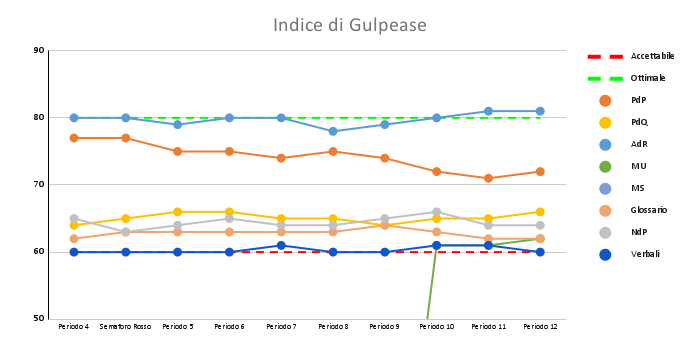
\includegraphics[scale=0.60]{Indice di Gulpease.png}
      \caption{Indice di Gulpease per documento per periodo}
    \end{figure}

  \subsection{Verifica del software}
    \subsubsection{Tempo medio di risposta}
    \begin{figure}[H]
      \centering
      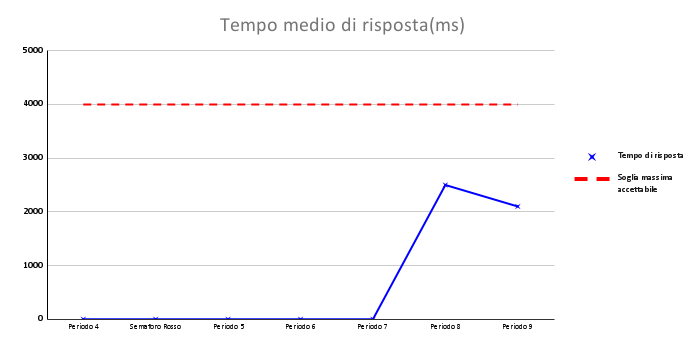
\includegraphics[scale=0.60]{Tempo medio di risposta(ms).png}
      \caption{Tempo medio di risposta dell'applicazione(ms)}
    \end{figure}


  \subsection{Verifica dei processi}
    \subsubsection{Estimated at Completion}
    \begin{figure}[H]
      \centering
      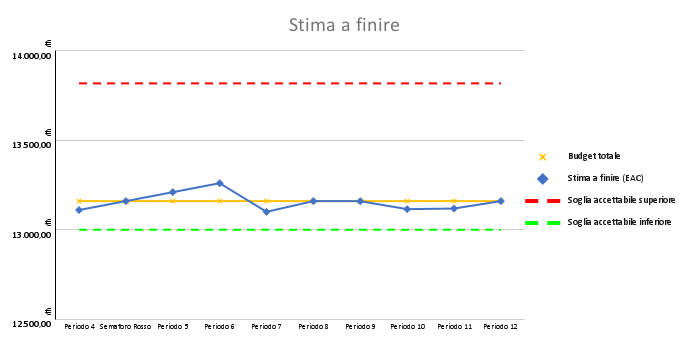
\includegraphics[scale=0.60]{Stimaafinire2.png}
      \caption{Valore stimato per la realizzazione del progetto}
    \end{figure}

    \subsubsection{Actual Cost e Estimate to Complete}
    \begin{figure}[H]
      \centering
      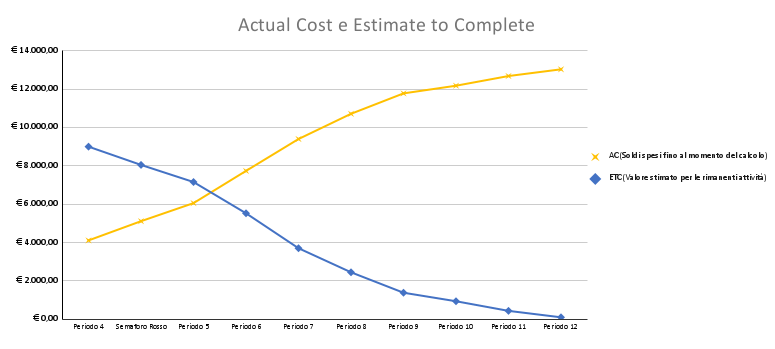
\includegraphics[scale=0.60]{Actual Cost e Estimate to Complete.png}
      \caption{Costo effettivamente sostenuto e valore stimato per la realizzazione delle rimanenti attività}
    \end{figure}

    \subsubsection{Earned Value e Planned Value}
    \begin{figure}[H]
      \centering
      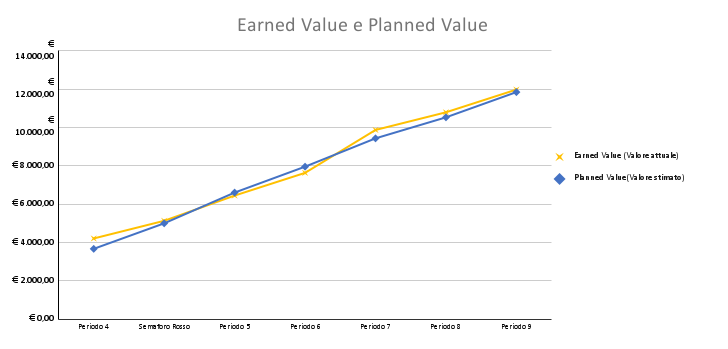
\includegraphics[scale=0.60]{Earned Value e Planned Value.png}
      \caption{Valore delle attività realizzate e costo pianificato per realizzare le rimanenti}
    \end{figure}

    \subsubsection{Schedule Variance e Budget Variance}
    \begin{figure}[H]
      \centering
      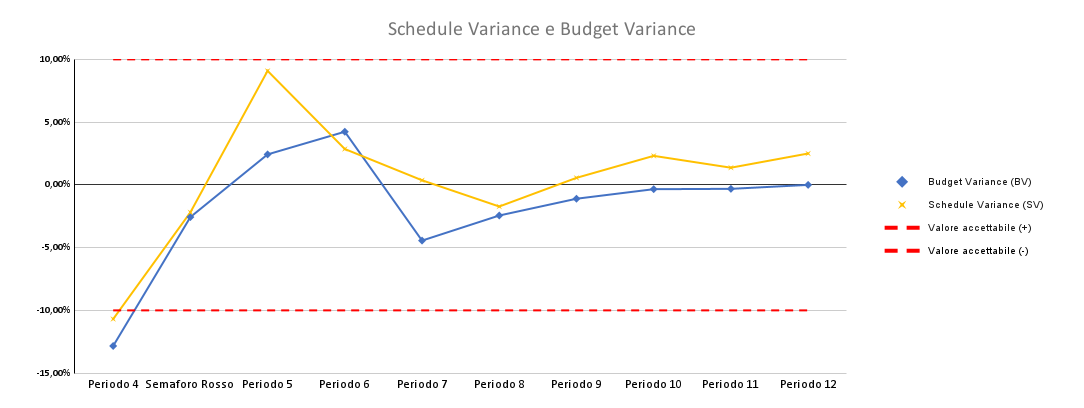
\includegraphics[scale=0.48]{Schedule Variance e Budget Variance.png}
      \caption{Schedule Variance e Budget Variance per incremento}
    \end{figure}

    \subsubsection{Copertura e stabilità dei requisiti}
    \begin{figure}[H]
      \centering
      \includegraphics[scale=0.60]{Indice di Stabilità dei Requisiti e Requisiti Obbligatori Soddisfatti.png}
      \caption{Percentuale di copertura e stabilità dei requisiti}
    \end{figure}

    \subsubsection{Metriche soddisfatte}
    \begin{figure}[H]
      \centering
      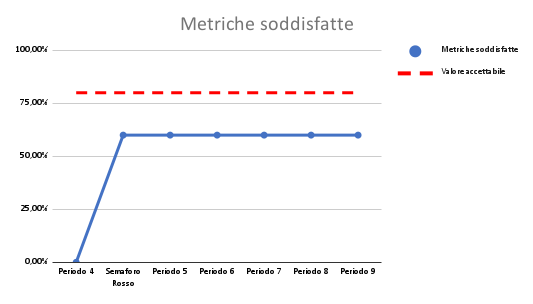
\includegraphics[scale=0.60]{Metriche soddisfatte.png}
      \caption{Percentuale di metriche di qualità soddisfatte}
    \end{figure}

    \subsubsection{Facilità di utilizzo}
    \begin{figure}[H]
      \centering
      \includegraphics[scale=0.60]{Facilità di utilizzo(click).png}
      \caption{Facilità di utilizzo espressa in click}
    \end{figure}

    \subsubsection{Comprensibilità codice}
    \begin{figure}[H]
      \centering
      \includegraphics[scale=0.48]{Comprensibilità codice.png}
      \caption{Percentuale di Comprensibilità del codice}
    \end{figure}

    \subsubsection{Browser supportati}
    \begin{figure}[H]
      \centering
      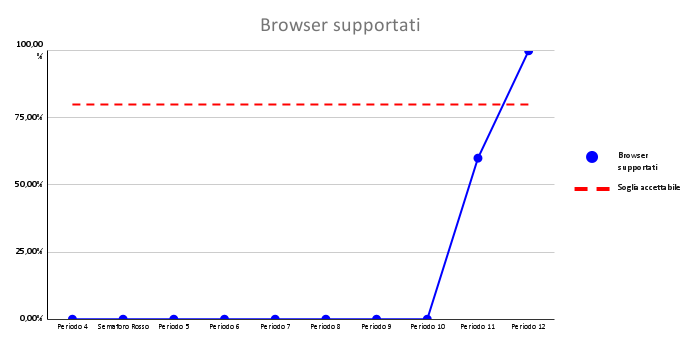
\includegraphics[scale=0.60]{Browser supportati.png}
      \caption{Percentuale di browser supportati sul totale}
    \end{figure}

    \subsubsection{Code coverage e percentuale di test superati/falliti}
    \begin{figure}[H]
      \centering
      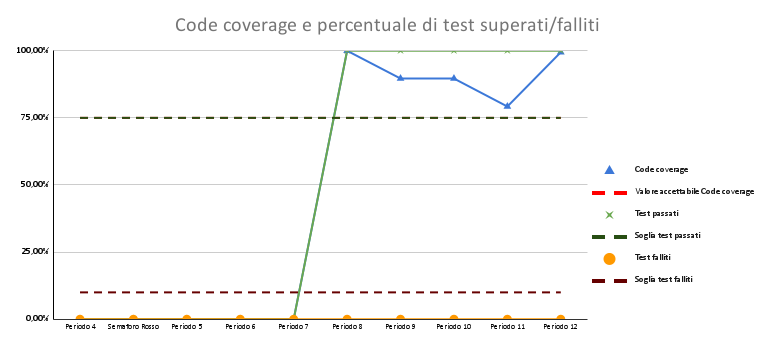
\includegraphics[scale=0.60]{Code coverage e percentuale di test superati_falliti2.png}
      \caption{Copertura del codice e percentuale di test superati e falliti per incremento. In questo grafico non sono presenti i file drawer.}
    \end{figure}

    \subsubsection{Copertura dei test}
    \begin{figure}[H]
      \centering
      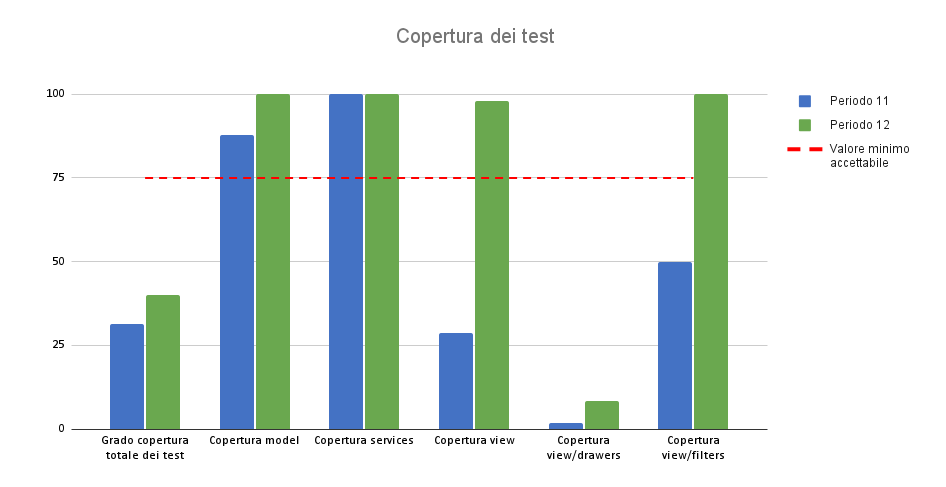
\includegraphics[scale=0.50]{Copertura dei test.png}
      \caption{Copertura offerta dai test per ogni componente}
    \end{figure}

    \begin{figure}[H]
      \centering
      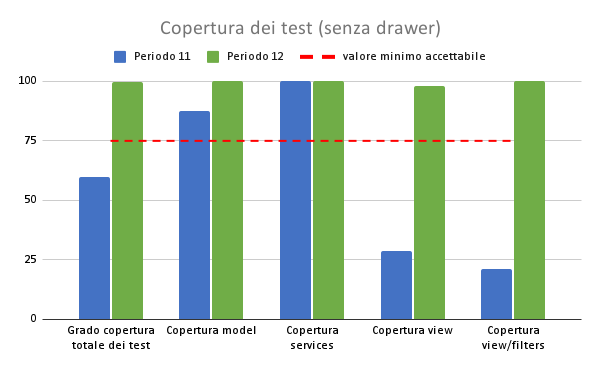
\includegraphics[scale=0.60]{Copertura dei test (senza drawer).png}
      \caption{Copertura offerta dai test trascurando la componente "drawer"}
    \end{figure}

    \subsubsection{Numero di test per componente}
    \begin{figure}[H]
      \centering
      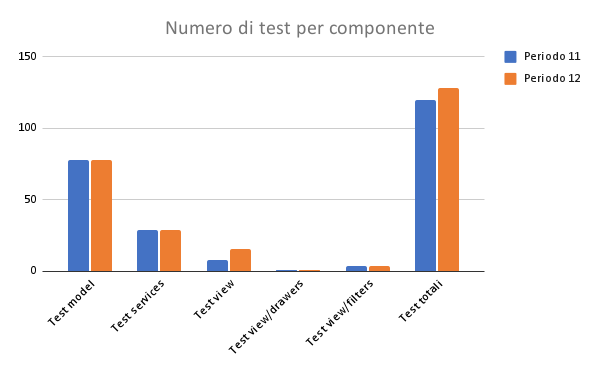
\includegraphics[scale=0.60]{Numero di test per componente.png}
      \caption{Numero di test per componente}
    \end{figure}

    \subsubsection{Test sul totale per ogni componente}
    \begin{figure}[H]
      \centering
      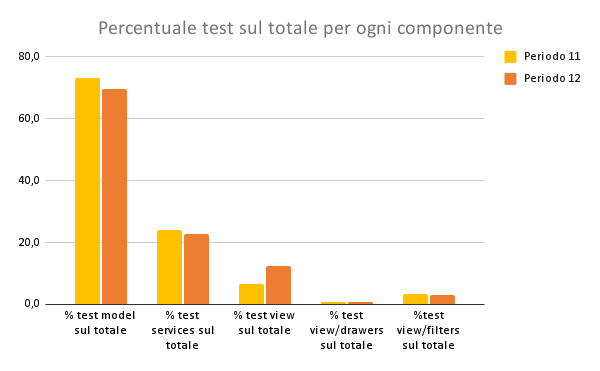
\includegraphics[scale=0.60]{Percentuale test sul totale per ogni componente.png}
      \caption{Percentuale di test sul totale per ogni componente}
    \end{figure}

  \chapter{Valutazioni per il miglioramento}
 In questa sezione il team riporta le criticità riscontrate durante
 lo svolgimento del progetto al fine di migliorare la qualità del
 lavoro svolto.

\section{Valutazione sull'organizzazione}
\begin{longtable}{|p{0.16\linewidth}|p{0.11\linewidth}|p{0.3\linewidth}|p{0.3\linewidth}|}
    \hline
    \rowcolor[HTML]{036400}
    {\color[HTML]{FFFFFF} \textbf{Problema}} & {\color[HTML]{FFFFFF} \textbf{Gravità}} & {\color[HTML]{FFFFFF} \textbf{Descrizione}} & {\color[HTML]{FFFFFF} \textbf{Soluzione}} \\ \hline
    \rowcolor[HTML]{EFEFEF}
    Suddivisione compiti& Bassa & Inizialmente è stato deciso di suddividere il gruppo in sottogruppi e assegnare a ciascuno di essi un documento differente da redarre. Questa scelta si è rivelata svantaggiosa a causa della dipendenza tra alcuni documenti che impediva il lavoro parallelo dei sottogruppi. & Il gruppo ha deciso di convergere le proprie forze per la realizzazione sequenziale dei documenti con dipendenza. \\ \hline
    \rowcolor[HTML]{C0C0C0}
    Organizzativo & Bassa  & Durante il periodo della seconda milestone, dal 20/12/21 al 10/01/22, il gruppo si è reso conto di non essere in grado di rispettare le ore preventivate. &Il gruppo ha consuntivato meno ore rispetto a quelle preventivate. Inoltre per evitare che tale errore possa ripetersi si è deciso di porre maggior attenzione nell'attività di previsione oraria, andando a segnalare le ore che si è sicuri verranno impiegate per l'avanzamento delle attività di progetto.  \\ \hline
    \rowcolor[HTML]{EFEFEF}
    Organizzativo & Media & Durante il periodo della terza milestone, dal 15/01/2022 al 04/02/2022, il gruppo si è reso conto di non essere in grado di rispettare le ore preventivate. La presenza della sessione d'esame ha occupato più tempo del previsto e la stima di disponibilità oraria è risultata quindi errata. & Il gruppo ha consuntivato meno ore rispetto a quelle preventivate. Per evitare che questa situazione possa ripresentarsi, visto che è già la seconda volta, il gruppo ha capito che deve prestare ancora più attenzione nell'attività di previsione oraria, cercando di prevedere quali potrebbero essere le problematiche che possono presentarsi durante il periodo.  \\ \hline
    \rowcolor[HTML]{C0C0C0}
    Resoconto attività di verifica & Media & Fino a poco prima della revisione RTB il gruppo non ha controllato il progresso dei documenti utilizzando le metriche che si era posto di sfruttare. In questo modo, in prossimità della revisione, è stato impossibile poter modificare in modo adeguato i documenti per renderli il più conformi possibile a quanto inizialmente prestabilito. & Il gruppo ha deciso di svolgere i dovuti controlli ai documenti ad ogni termine delle milestone, indicativamente ogni due settimane, in modo da avere una visione più chiara del loro sviluppo.\\ \hline
    \hline
\end{longtable}



\section{Valutazione sui ruoli}
\begin{table}[H]
    \centering
    \begin{tabular}{|p{0.16\linewidth}|p{0.11\linewidth}|p{0.3\linewidth}|p{0.3\linewidth}|}
   \hline
    \rowcolor[HTML]{036400}
    {\color[HTML]{FFFFFF} \textbf{Problema}} & {\color[HTML]{FFFFFF} \textbf{Gravità}} & {\color[HTML]{FFFFFF} \textbf{Descrizione}} & {\color[HTML]{FFFFFF} \textbf{Soluzione}} \\ \hline
    \rowcolor[HTML]{EFEFEF}
    Responsabile & Media & Inizialmente il gruppo ha incontrato svariate difficoltà nella distribuzione delle ore e nella suddivisione equa dei compiti. & Il gruppo ha deciso di puntare a previsioni di più breve durata. \\ \hline
    \rowcolor[HTML]{C0C0C0}
    Verificatore & Bassa & Nelle fasi iniziali del progetto il ruolo è stato svolto con superficialità, causando un incremento degli errori nei documenti. & Il gruppo ha deciso di porre maggior attenzione e tempo nelle attività di verifica. \\ \hline
    \end{tabular}
\end{table}


\section{Valutazione sugli strumenti di lavoro}
    \begin{table}[H]
        \centering
        \begin{tabular}{|p{0.16\linewidth}|p{0.11\linewidth}|p{0.3\linewidth}|p{0.3\linewidth}|}
        \hline
        \rowcolor[HTML]{036400}
        {\color[HTML]{FFFFFF} \textbf{Problema}} & {\color[HTML]{FFFFFF} \textbf{Gravità}} & {\color[HTML]{FFFFFF} \textbf{Descrizione}} & {\color[HTML]{FFFFFF} \textbf{Soluzione}} \\ \hline
        \rowcolor[HTML]{EFEFEF}
        GitHub & Bassa & Inizialmente alcuni membri del gruppo hanno riscontrato difficoltà nell'utilizzo dello strumento di versionamento a causa dell'inesperienza. & I membri del gruppo con le lacune hanno svolto un'attività di autoapprendimento utilizzando anche le risorse fornite dai compagni più esperti. \\ \hline
        \rowcolor[HTML]{C0C0C0}
        \LaTeX & Media & L'utilizzo del software si è dimostrata più complessa di quanto ci si aspettasse, in particolare per quanto riguarda il posizionamento delle immagini e delle tabelle. & Il gruppo ha investito una maggior quantità di tempo nelle attività di autoapprendimento per comprendere meglio il funzionamento dello strumento in questione. \\ \hline
        \end{tabular}
    \end{table}

\end{document}
